\documentclass[tikz,border=0pt]{standalone}
\usepackage[T1]{fontenc}
\usepackage{tgheros}
\usepackage{newtxmath}
\usepackage{amsmath}
\usetikzlibrary{arrows.meta}
\definecolor{ink}{HTML}{172C3D}
\definecolor{muted}{HTML}{526674}
\definecolor{edge}{HTML}{B9C9D4}
\definecolor{teal}{HTML}{147D75}
\definecolor{tea}{HTML}{EAF6F3}
\definecolor{amber}{HTML}{9B5C21}
\definecolor{cream}{HTML}{FFF4E7}
\definecolor{bluegray}{HTML}{EDF3F8}
\renewcommand{\familydefault}{\sfdefault}

\begin{document}
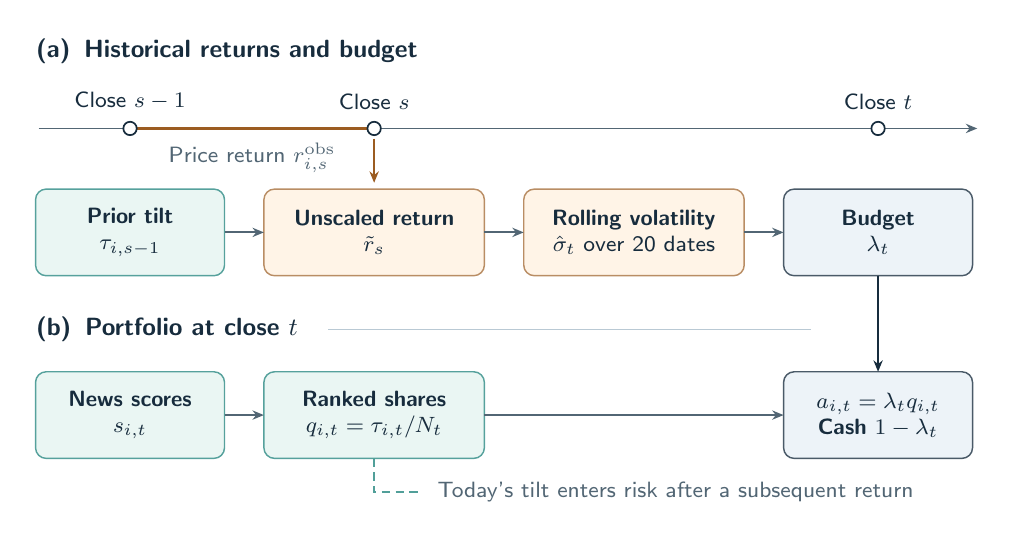
\begin{tikzpicture}[
  x=1mm,y=1mm,text=ink,font=\sffamily\fontsize{8.5}{10}\selectfont,
  flow/.style={-{Stealth[length=1.45mm,width=1.18mm]},line width=.66pt,draw=muted},
  news/.style={card,draw=teal!72,fill=tea},
  risk/.style={card,draw=amber!70,fill=cream},
  joint/.style={card,draw=ink!78,fill=bluegray},
  card/.style={rounded corners=1.35mm,inner sep=1.25mm,outer sep=0pt,
    minimum height=11mm,align=center,line width=.52pt,draw},
  heading/.style={anchor=west,inner sep=0pt,font=\sffamily\bfseries\fontsize{9.5}{11}\selectfont},
  axislabel/.style={font=\sffamily\fontsize{8.0}{9.6}\selectfont,inner sep=0pt},
  detail/.style={font=\sffamily\fontsize{8.0}{9.6}\selectfont,text=muted,inner sep=0pt}
]
\path[use as bounding box] (0,0) rectangle (122,-62.3);
\node[heading] at (1,-3.05) {\textbf{(a)}\enspace Historical returns and budget};

% Each observation pairs the prior panel tilt with a price return ending at s.
\draw[flow] (1.4,-12.8) -- (120.6,-12.8);
\draw[amber,line width=1.35pt] (13,-12.8) -- (44,-12.8);
\foreach \x/\labeltext in {13/$s-1$,44/$s$,108/$t$} {
  \draw[ink,fill=white,line width=.62pt] (\x,-12.8) circle[radius=.85mm];
  \node[axislabel,anchor=south] at (\x,-10.5) {Close \labeltext};
}
\node[detail] at (28.5,-16.55) {Price return $r^{\mathrm{obs}}_{i,s}$};
\draw[flow,draw=amber] (44,-14.1) -- (44,-19.7);

\node[news,minimum width=24mm] (prior) at (13,-26.0)
  {\textbf{Prior tilt}\\[-.06em]$\tau_{i,s-1}$};
\node[risk,minimum width=28mm] (realized) at (44,-26.0)
  {\textbf{Unscaled return}\\[-.06em]$\tilde r_s$};
\node[risk,minimum width=28mm] (rolling) at (77,-26.0)
  {\textbf{Rolling volatility}\\[-.06em]$\hat\sigma_t$ over 20 dates};
\node[joint,minimum width=24mm] (budget) at (108,-26.0)
  {\textbf{Budget}\\[-.06em]$\lambda_t$};
\draw[flow] (prior) -- (realized);
\draw[flow] (realized) -- (rolling);
\draw[flow] (rolling) -- (budget);

\node[heading] at (1,-38.3) {\textbf{(b)}\enspace Portfolio at close $t$};
\draw[edge,line width=.52pt] (38.2,-38.3) -- (99.5,-38.3);

% The current rank tilt and the already-computed budget meet at execution.
\node[news,minimum width=24mm] (scores) at (13,-49.2)
  {\textbf{News scores}\\[-.06em]$s_{i,t}$};
\node[news,minimum width=28mm] (tilt) at (44,-49.2)
  {\textbf{Ranked shares}\\[-.06em]$q_{i,t}=\tau_{i,t}/N_t$};
\node[joint,minimum width=24mm] (allocation) at (108,-49.2)
  {$a_{i,t}=\lambda_t q_{i,t}$\\[-.06em]\textbf{Cash} $1-\lambda_t$};
\draw[flow] (scores) -- (tilt);
\draw[flow] (tilt) -- (allocation);
\draw[flow,draw=ink] (budget) -- (allocation);

\draw[teal!74,line width=.55pt,densely dashed] (44,-54.7) |- (50,-59.0);
\node[detail,anchor=west] at (52,-59.0)
  {Today's tilt enters risk after a subsequent return};
\end{tikzpicture}
\end{document}
